\documentclass[../dissertation.tex]{subfiles}
\begin{document}

\chapter{Research}
\label{sec:research}

\section{Background}
\label{sec:background}

Initial research was completed over a three month period and covered network visualisation, specifically massive network visualisation, and additionally looked into software that existed which visualised networks. The dearth of previous research confirmed that this is an area that was worth exploring further. This meant that exploration had to be done from scratch as there was no previous studies to build upon. However, this proved advantageous as the wealth of information gained during this period informed future decisions throughout the project.

In regards to the visualisation of massive networks, some important techniques learnt were:

\subsection{Node bundling}
\label{sec:node_bundling}
This is when software uses algorithms to decide (with or without some form of user input) which nodes are very similar to each other, and upon establishing this relationship, groups them in to one node, generally visually different in some way (often by size or colour). It ``creates a less complicated visualization without losing connectivity information by automatically abstracting small [...] subgraphs'' \cite{six2003effective}. This allows for hundreds or thousands of nodes to be grouped into one node and hence take up for less memory, processing power, bandwidth and screen space on the users machine. A way to make this even more helpful is to show how the nodes being bundled interact with themselves, for example if they are heavily connected or all connected to just a few nodes, or if they are in a ring formation. See Figure \ref{fig:bundling} for an example of both node and edge bundling.
    
\subsection{Edge bundling}
\label{sec:edge_bundling}
This is similar to node bundling but applied to edges. It ``trade[s] clutter for overdraw by routing related edges along similar paths'' \cite{hurter2012graph}, and ``can be seen as sharpening the edge spatial density, by making it high along bundles and low elsewhere'' \cite{hurter2012graph}. If node bundling is done then this process will have less of an impact as all of the edges will already be bundled together, assuming the node bundling algorithm was optimal. Like node bundling, it is often shown through the change of the size of the edge or the colour. See Figure \ref{fig:bundling} for an example of both node and edge bundling.
\begin{figure}
    \centering
    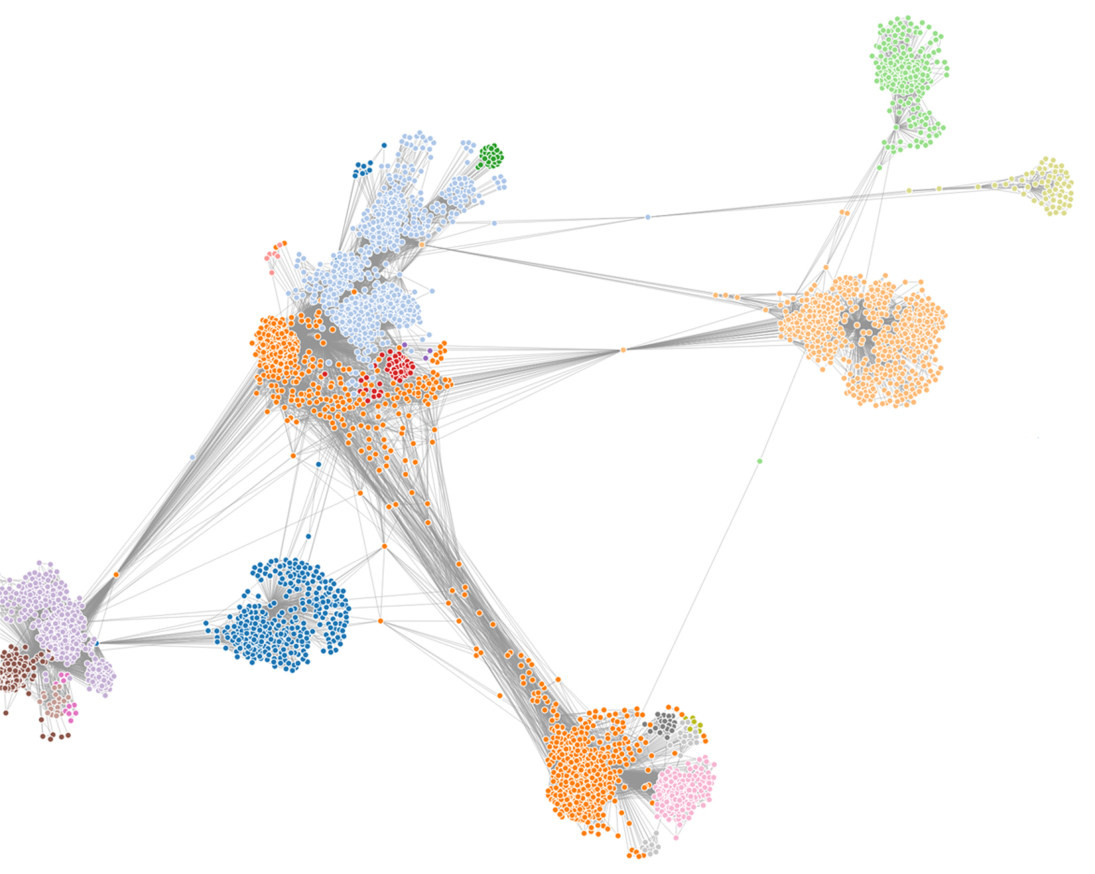
\includegraphics[width=12cm]{4/bundling1}
    \\$\downarrow$\\
    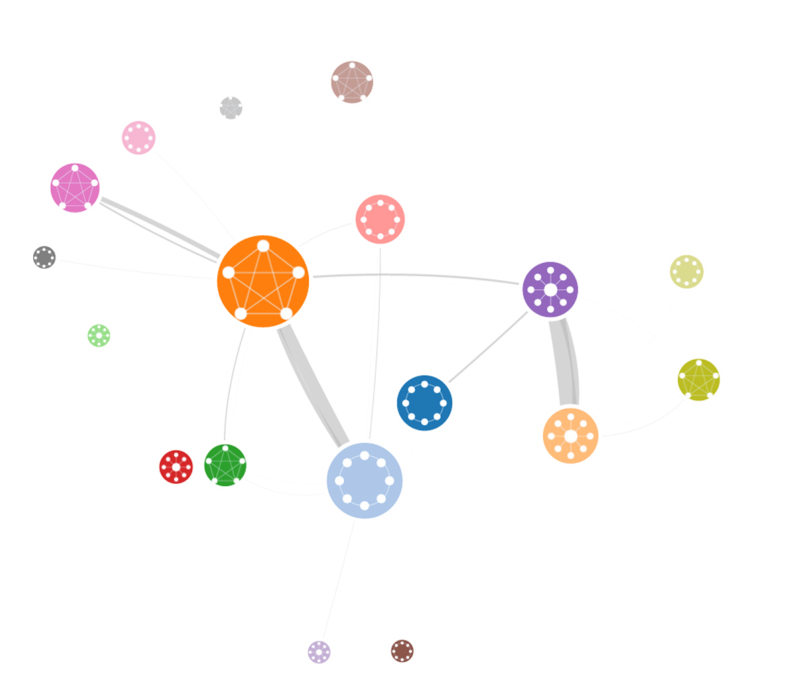
\includegraphics[width=12cm]{4/bundling2}
    \caption{Demonstrates both node and edge bundling, where thickness of edge displays how many edges there are, and size of node indicates number of nodes group. On top of that, each node displays how nodes within it were connected together. This particular example displays a comparison between a common network visualisation and a ModulGraph-based network visualisation. \cite{li2015modulgraph}}
    \label{fig:bundling}
\end{figure}

\subsection{Local Edge Lens}
This involves rendering all or part of the network, and upon focusing on a section of the network, that part is zoomed in or clarified as if through a lens and that part of the network is zoomed in, becoming more clear. Another way of implementing this can be that when the lens is applied, it can render more information that was not shown before in order to save computational power. ``By doing so, the cluttering of edges is removed for a local focus region defined by the position and scope of the lens'' \cite{tominski2006fisheye} See Figure \ref{fig:local}.
\begin{figure}
    \centering
    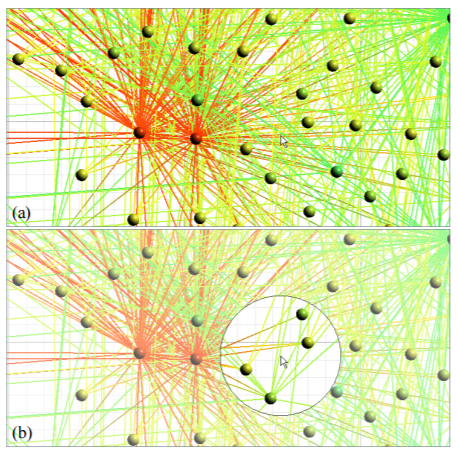
\includegraphics[width=8cm]{4/local}
    \caption{If a network is cluttered (a), then it can be hard to get useful information from it. A local edge lens (b) lets users easily identify which edges are connected to which nodes. \cite{tominski2006fisheye}}
    \label{fig:local}
\end{figure}

\subsection{Deleting unnecessary content smartly}
This involves using an algorithm to remove certain nodes or edges that are deemed to be adding little or no useful information for the user. This algorithm can take no parameters, which would then make it a variant on Node/Edge bundling, or work off a user's input, in which they specify what they are interested in, so other information is partially or fully removed. It differs to Node and Edge Bundling as a result of the amount of information that is removed, which is far greater in this case. See Figure \ref{fig:deletion}. 
\begin{figure}
    \centering
    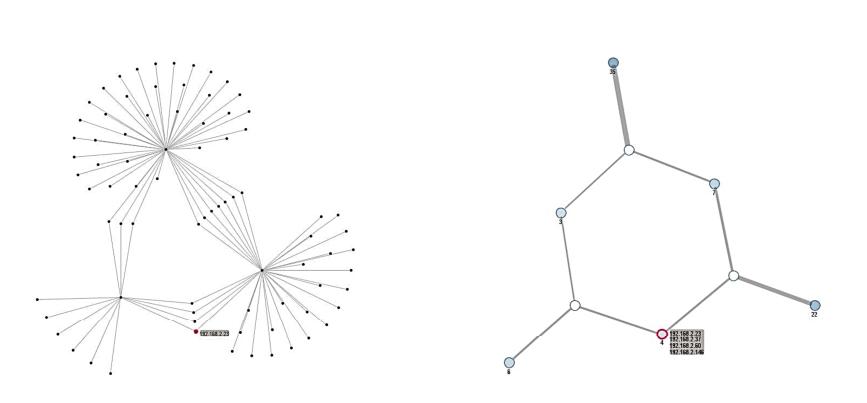
\includegraphics[width=15cm]{4/deletion}
    \caption{This figure clearly shoes how the deletion of many nodes mean that, although information is lost, the visualisation can become more clear as a result of the operation. \cite{hu2015visualizing}}
    \label{fig:deletion}
\end{figure}

\section{Current Network Visualisation Software}

On top of finding out techniques used by software for large network visualisation, a list was also created of all software that was mentioned in papers or found during research that was related to large network visualisation. Quite often, the software mentioned had been hand-made for that project and was not feature complete, or the software could only be used for a price, but the below list contains the names of software that seemed reasonable to look further into, found by searching online and through mentions from papers:
\begin{itemize}
    \item GUESS \cite{guess}
    \item SNAP \cite{snap}
    \item Gephi \cite{gephi}
    \item GraphViz \cite{graphviz}
    \item Tulip \cite{tulip}
    \item D3.js \cite{d3}
    \item Vis.js \cite{vis}
\end{itemize}

This software is reviewed in Chapter \ref{sec:systematic-review}, below.

\end{document}